\documentclass[tikz]{standalone}
\usetikzlibrary{calc,positioning, backgrounds,fit,shapes.geometric}


\begin{document}
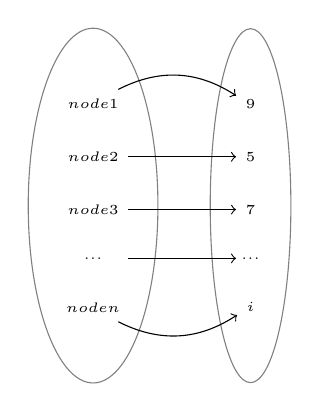
\begin{tikzpicture}[every node/.style={}]

\begin{scope}[node distance=0.3cm]
\node(n1) {\tiny $node 1$};
\node(n2) [below=of n1] {\tiny $node 2$};
\node(n3) [below=of n2]{\tiny $node 3$};
\node(n4) [below=of n3] {\tiny $...$};
\node(n5) [below=of n4]{\tiny $node n$};
\end{scope}

\begin{scope}[on grid, node distance=2cm]
\node(t1) [right=of n1]{\tiny $9$};
\node(t2) [right=of n2]{\tiny $5$};
\node(t3) [right=of n3]{\tiny $7$};
\node(t4) [right=of n4]{\tiny $...$};
\node(t5) [right=of n5]{\tiny $i$};
\end{scope}

\begin{scope}[on background layer]
\node[ellipse,draw, gray, fit=(n1)(n2)(n3)(n4)(n5)]{};
\node[ellipse,draw, gray, fit=(t1)(t2)(t3)(t4)(t5)]{};
\end{scope}

\draw[->] (n1) to[bend left]  (t1);
\draw[->] (n2) to (t2);
\draw[->] (n3) to (t3);
\draw[->] ($(n4.east)!(n3.east)!(t4.west)$) to ($(n4.east)!(t3.west)!(t4.west)$);
\draw[->] (n5) to[ bend right] (t5);

 
\end{tikzpicture}
\end{document}
